% ---------------------------------------------------------------------------
%  Panel captions for "A Circuit Model of the Cell as a Constructor of
%  Causal Knowledge Graphs".
%
%  Every number quoted below is read from ckg/validation/results/*.json and is
%  reproducible by  python run_validation.py  followed by  python make_figures.py.
%  Requires: graphicx, siunitx, and the \Sk \St \Se \pan macros from the main
%  preamble. Figures are referenced as figures/panel_*.pdf; adjust the path or
%  set \graphicspath if this file is included from another directory.
% ---------------------------------------------------------------------------

\begin{figure*}[!htbp]
    \centering
    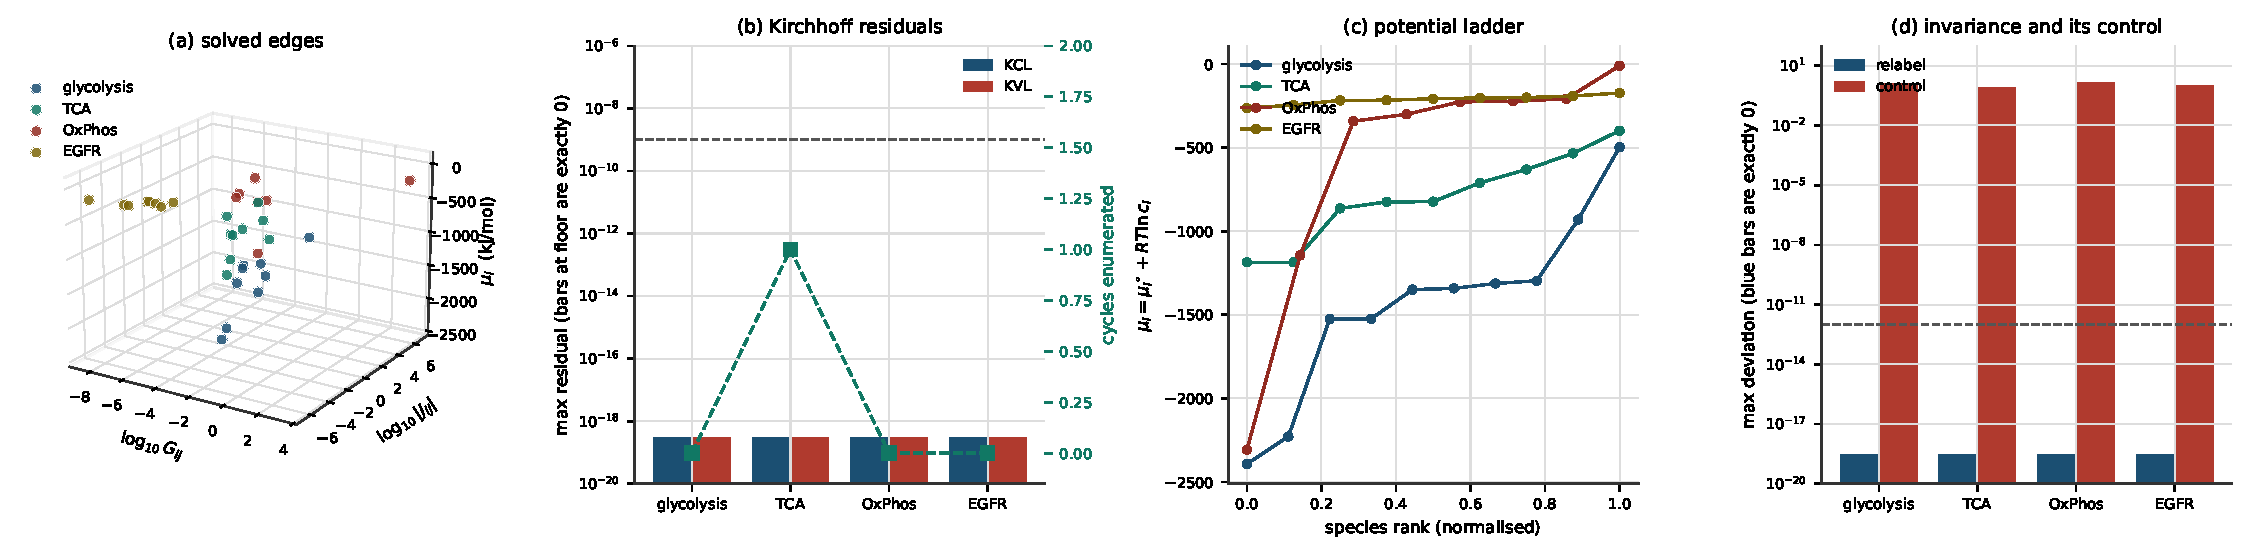
\includegraphics[width=\textwidth]{figures/panel_1_circuit.pdf}
    \caption{\textbf{The circuit layer: Kirchhoff correspondence and the invariance of the contact map.}
    All four networks are solved at steady state under $\mu_i = \mu_i^\circ + RT\ln c_i$ with $RT = \SI{2.577}{\kilo\joule\per\mole}$ at \SI{310}{\kelvin}, and every quantity plotted is a solved circuit variable rather than a schematic.
    (\textbf{A})~Every solved edge of all four networks in $(\log_{10} G_{ij},\ \log_{10}|J_{ij}|,\ \mu_i)$. Conductances span roughly fourteen decades, so the recovered circuit is strongly stiff: a handful of edges carry the conductance while the remainder are effectively open, which is why a budgeted traversal is a meaningful constraint rather than a formality.
    (\textbf{B})~Kirchhoff residuals per network on a logarithmic axis. Every KCL and KVL residual is \emph{exactly} zero, so all bars are drawn at the plotting floor and the axis label states this; a logarithmic axis cannot render zero, and a bar of visible height here would be an artefact of the plot rather than a result. The right-hand axis carries the number of simple directed cycles enumerated, and it records the coverage limitation of this check honestly: only the citric-acid cycle contributes a cycle ($1$; the other three contribute $0$), so the Wegscheider half of \Cref{thm:kirchhoff} is exercised on a single cycle and no more.
    (\textbf{C})~The potential ladder $\mu_i$ against normalised species rank. Glycolysis and the citric-acid cycle descend across $\sim\!\SI{2000}{\kilo\joule\per\mole}$, while the EGFR/MAPK cascade is nearly flat --- a signalling network carries information without a comparable potential drop.
    (\textbf{D})~The invariance of \Cref{prop:contact-determined} against the control that gives it content. Permuting species labels leaves the contact map deviation at exactly $0$ (blue bars, at the floor), while permuting the underlying concentrations rather than the labels moves it by $0.80$--$1.41$ (red). Without the second series the first could not fail, which is the discipline of \Cref{rem:control-refused}.}
    \label{fig:panel1}
\end{figure*}

\begin{figure*}[!htbp]
    \centering
    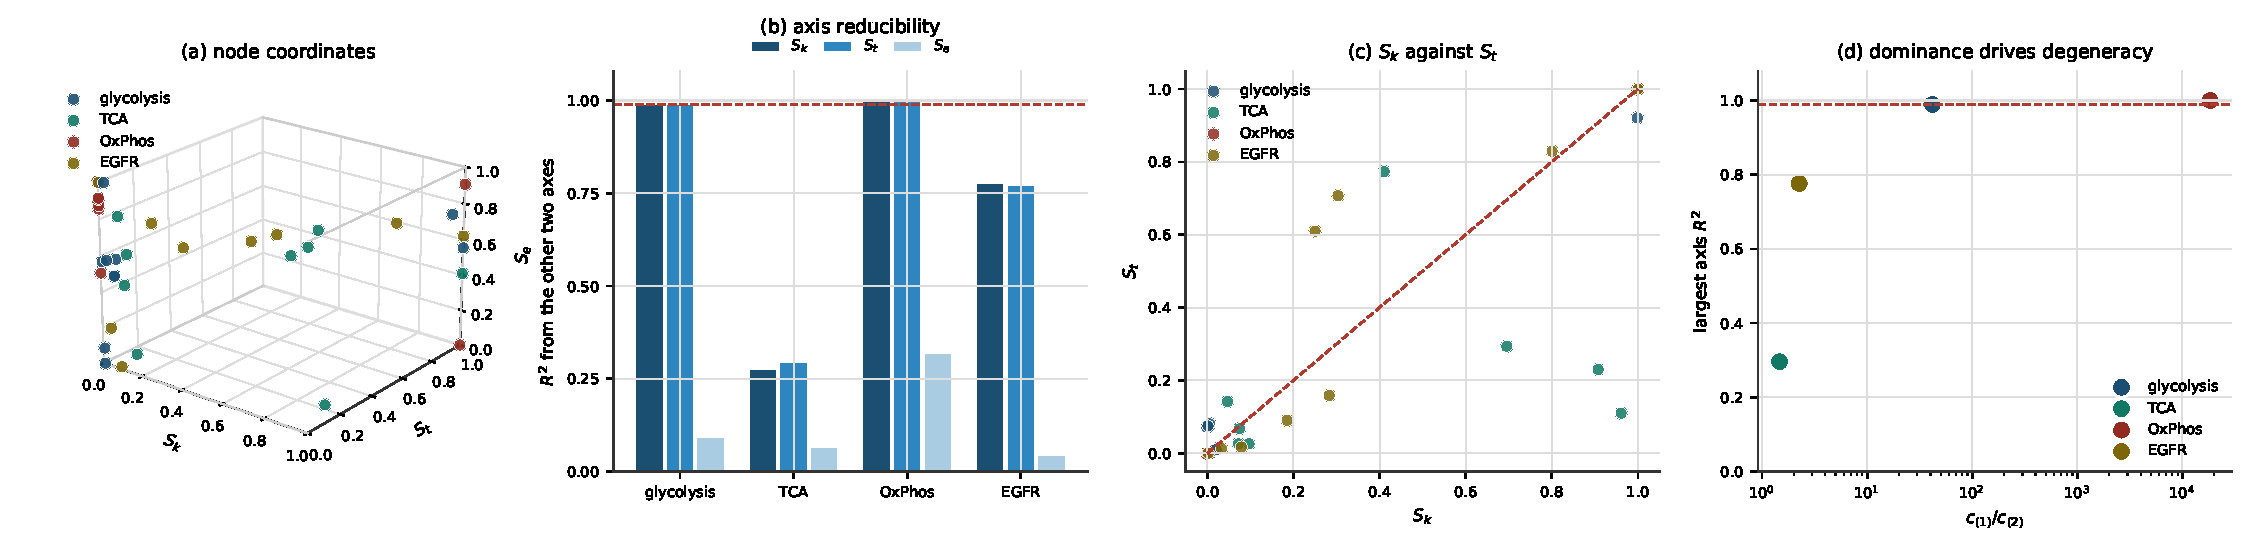
\includegraphics[width=\textwidth]{figures/panel_2_coordinate.pdf}
    \caption{\textbf{The node coordinate $\mathbf{S}: V \to [0,1]^{3}$, and the concentration regime in which it degenerates.}
    Each vertex is embedded at $(\Sk, \St, \Se)$ by normalising conductance sum, flux sum and chemical potential against network extrema.
    (\textbf{A})~Every species of all four networks in the unit cube. Occupancy is sparse and strongly clustered near the low-$\Sk$, low-$\St$ face: most species are ordinary, and a few dominate both normalisers.
    (\textbf{B})~Axis reducibility, measured as the $R^2$ of each axis regressed on the other two, with the $0.99$ line marked. Oxidative phosphorylation saturates at $R^2 = 1.000$ on both $\Sk$ and $\St$; glycolysis sits just under the line at $0.989$; the citric-acid cycle ($0.28$, $0.30$) and the EGFR/MAPK cascade ($0.78$, $0.77$) do not. The energetic axis $\Se$ stays low throughout ($0.045$--$0.32$) and is never the redundant one.
    (\textbf{C})~The oxidative-phosphorylation collinearity shown without a regression: $\St$ against $\Sk$ collapses onto a two-valued indicator instead of spreading over the square, so the address there carries about one axis of information rather than three.
    (\textbf{D})~The mechanism, and the reason this is a defect of the normalisation rather than of the networks. Largest axis $R^2$ against the concentration dominance ratio $c_{(1)}/c_{(2)}$ on a logarithmic axis. Degeneracy tracks dominance monotonically: oxidative phosphorylation carries water at $c_{(1)}/c_{(2)} \approx 1.8\times10^{4}$ and glycolysis at $\approx 42$, and these are exactly the two networks whose coordinate collapses, while the citric-acid cycle ($1.5$) and the cascade ($2.3$) retain three independent axes. Since the coordinate divides by network extrema, a single dominating species flattens two of them. A practitioner should compute these regressions before trusting a three-axis address on a given network.}
    \label{fig:panel2}
\end{figure*}

\begin{figure*}[!htbp]
    \centering
    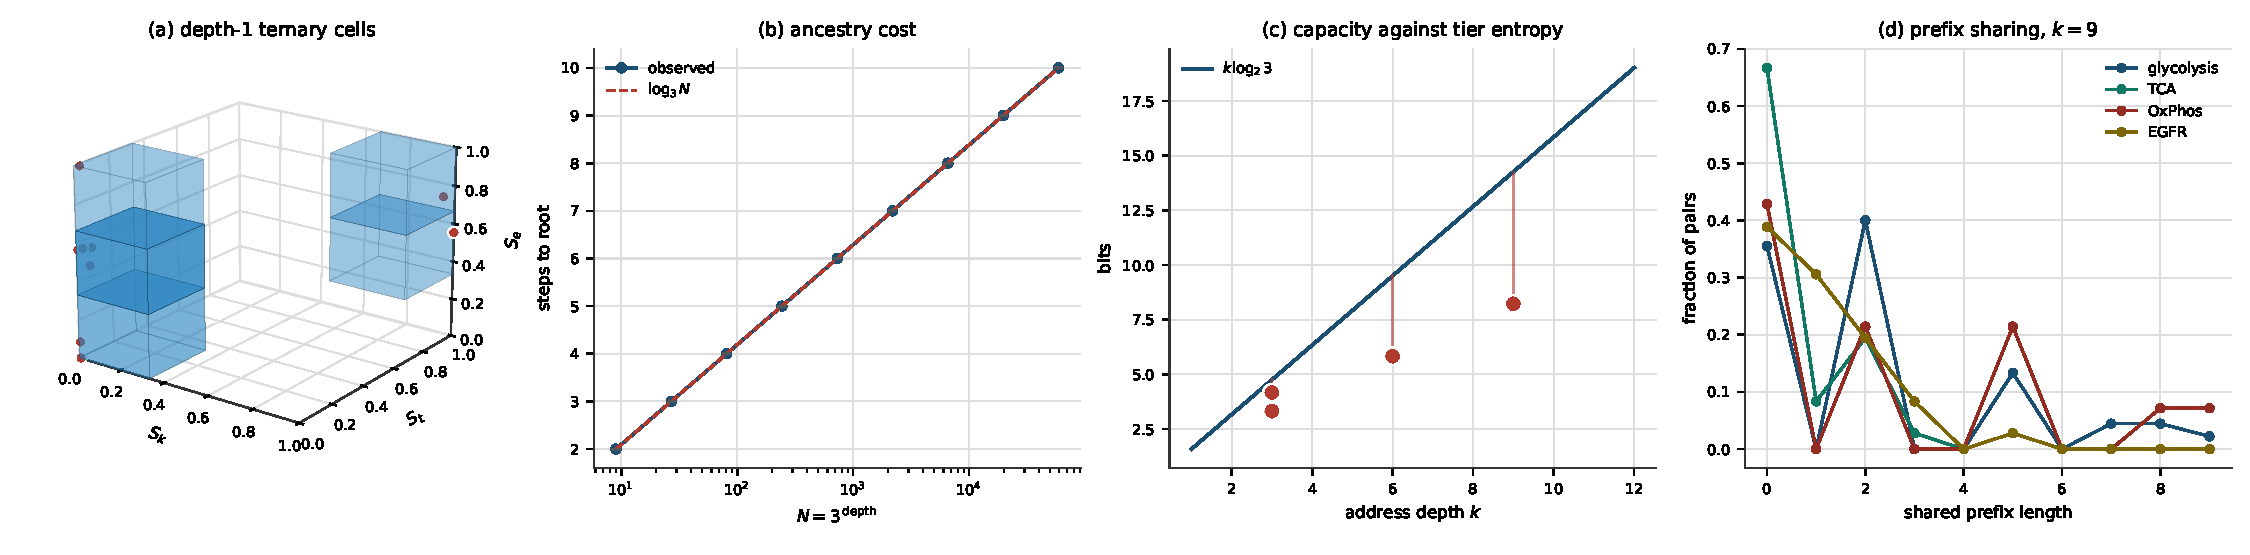
\includegraphics[width=\textwidth]{figures/panel_3_addressing.pdf}
    \caption{\textbf{Ternary addressing: ancestry as prefix arithmetic, with the trie never materialised.}
    Addresses are formed by interleaving the trit expansions of the three coordinate axes at depth $k = 3m$.
    (\textbf{A})~The depth-one ternary cells actually occupied by the four networks, drawn in the unit cube with opacity proportional to occupancy. The scheme partitions $[0,1]^3$ into $27$ cells at this depth, but the biology populates a small and uneven subset of them.
    (\textbf{B})~Ancestry cost. Observed steps to root against $N = 3^{\text{depth}}$ on a logarithmic abscissa, over depths $2$ through $10$ ($N = 9$ to $N = 59{,}049$). The observed count lies on $\log_3 N$ with \emph{zero} variance at every depth, and nearest common ancestor equals longest common prefix in every sampled pair --- \Cref{prop:notree}(ii) and (iii), computed from the address string alone with no structure traversed and none built.
    (\textbf{C})~Capacity $k\log_2 3$ against address depth, with the four tiers of the worked family plotted at their entropies. Every tier clears the bound of \Cref{prop:capacity} with slack: family ($18$ members, $H = 4.17$ bits, $k = 3$, margin $0.58$ bits), isoform ($57$, $5.83$, $k = 6$, margin $3.68$), allele ($300$, $8.23$, $k = 9$, margin $6.04$). The vertical stems are the unused margin, not error bars.
    (\textbf{D})~Distribution of shared prefix length over all species pairs at $k = 9$. Mass concentrates at short prefixes --- most pairs diverge within the first two symbols --- which is what makes a prefix comparison discriminating rather than a formality.}
    \label{fig:panel3}
\end{figure*}

\begin{figure*}[!htbp]
    \centering
    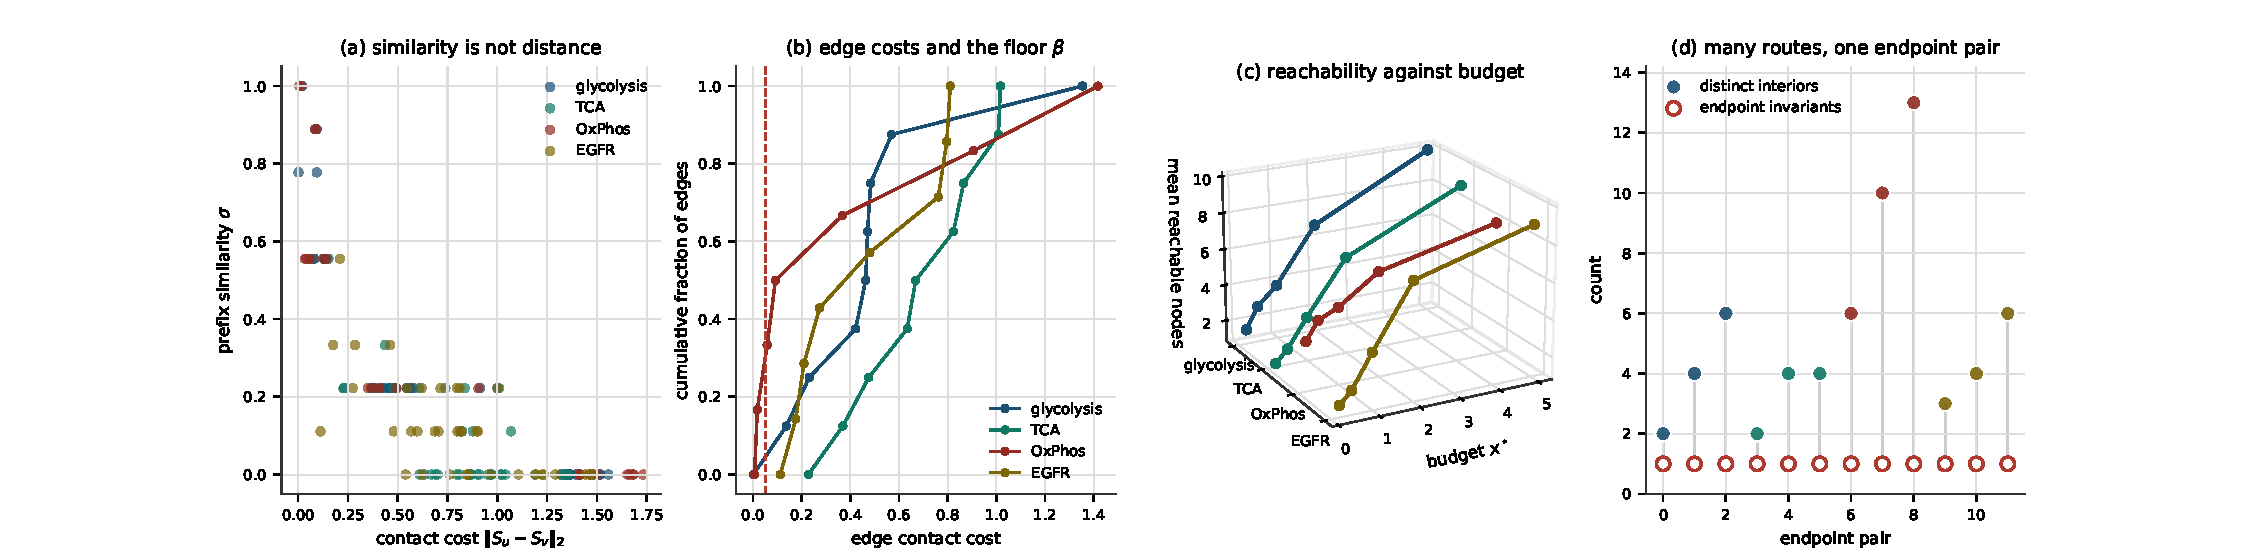
\includegraphics[width=\textwidth]{figures/panel_4_propagation.pdf}
    \caption{\textbf{Propagation under a contact budget, and the opacity of the interior route.}
    (\textbf{A})~Prefix similarity $\sigma$ against contact cost $\lVert S_u - S_v\rVert_2$ for every species pair in all four networks. The relation is emphatically not monotone: pairs at $\sigma = 0$ occur at every cost from $0.5$ to $1.75$, and pairs at nearly equal cost take values across most of the available range of $\sigma$. This is \Cref{rem:sigma-not-metric} shown on data --- $\sigma$ reports a shared partition cell, and reading it as a distance proxy is a category error.
    (\textbf{B})~Cumulative distribution of edge contact costs per network, with the contact floor $\beta = 0.05$ marked. The overwhelming majority of edges lie above the floor and the distributions differ markedly between networks, so a traversal budget binds differently in each.
    (\textbf{C})~Mean reachable nodes against budget $x^\star$, computed per network by budgeted expansion. Reachability rises with budget at a network-specific rate and saturates at different ceilings, confirming that the budget is a real constraint on propagation rather than a parameter without consequence.
    (\textbf{D})~For each endpoint pair, the number of distinct route interiors against the number of distinct endpoint invariants. Interiors proliferate --- up to $13$ for a single pair --- while the endpoint invariant stays at exactly $1$ for every pair tested ($90$ pairs in glycolysis, $72$ in the citric-acid cycle, $56$ in oxidative phosphorylation; opacity rate $1.0$ throughout). This is \Cref{thm:opacity}: the construction returns an equivalence class of routes, and increasing $k$ does not narrow it. Where the mechanism \emph{is} the scientific object, this is the wrong instrument.}
    \label{fig:panel4}
\end{figure*}

\begin{figure*}[!htbp]
    \centering
    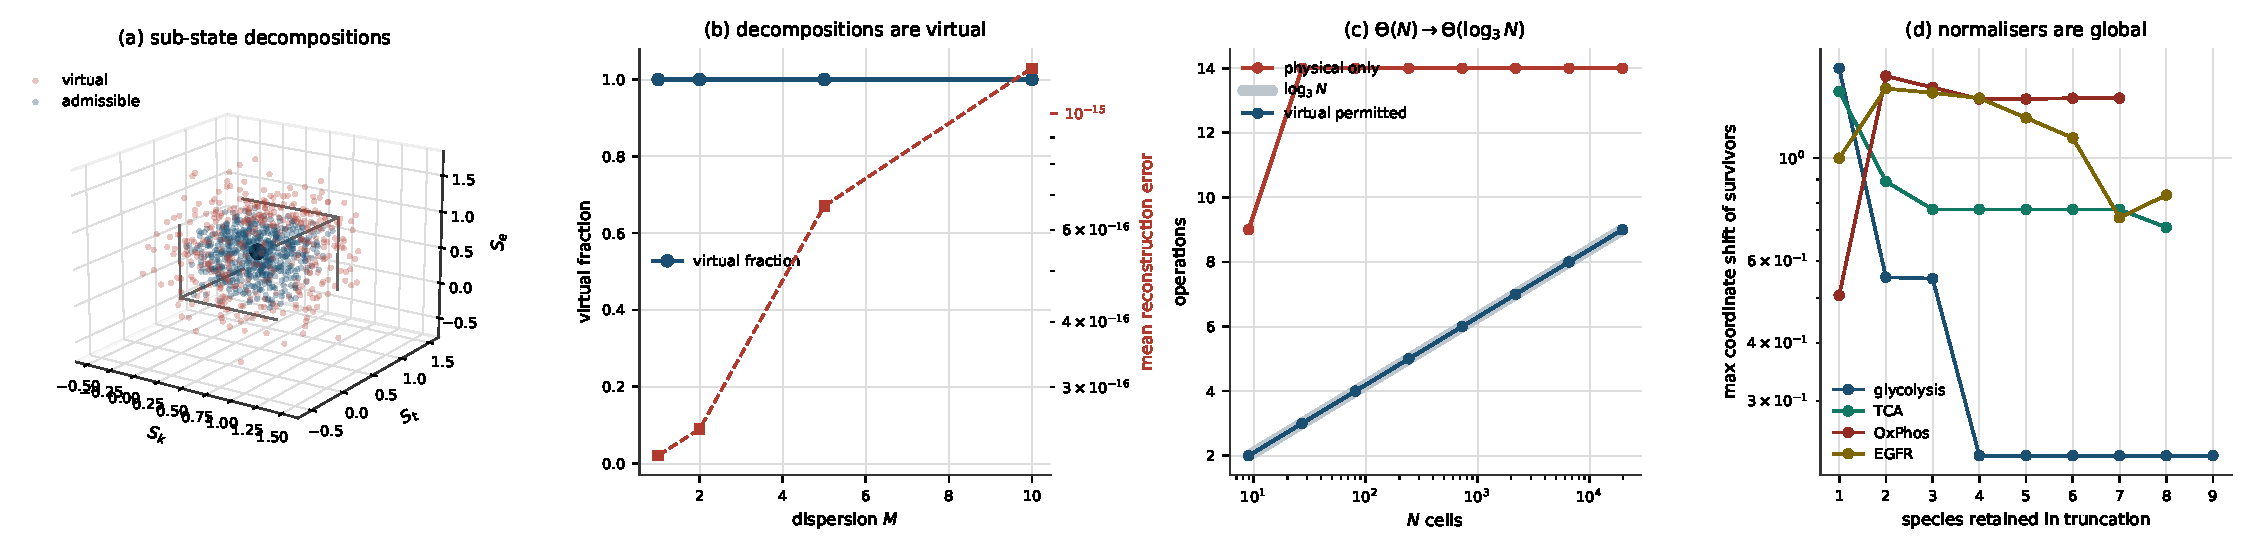
\includegraphics[width=\textwidth]{figures/panel_5_virtual.pdf}
    \caption{\textbf{Virtual sub-states: unphysical parts that average to a physical whole.}
    (\textbf{A})~One state (black) and its sub-state decompositions under $\tfrac{1}{p}\sum_r s_r = s$. Sub-states falling outside the unit cube (red) are virtual in the sense of \Cref{thm:collapse}: they are not themselves admissible coordinates, yet they average exactly onto one that is. Admissible sub-states (blue) are the minority.
    (\textbf{B})~Virtual fraction against dispersion $M$, with mean reconstruction error on the right-hand axis ($1000$ trials per point). The virtual fraction is $1.0$ at every dispersion tested --- \emph{every} decomposition is virtual, which is why the flat line is the result and not a plotting failure --- while reconstruction holds to $2.2\times10^{-16}$ at $M = 1$ and $1.2\times10^{-15}$ at $M = 10$. The averaging identity is exact while the parts are unphysical.
    (\textbf{C})~The collapse of \Cref{cor:speedup}. Operations against $N$ cells with $N$ logarithmic. Permitting virtual sub-states tracks $\Theta(\log_3 N)$ --- drawn as the wide grey underlay, which the measured series lies on exactly --- while the physical-only count saturates at $14$ and cannot descend further, a ratio that grows without bound in $N$.
    (\textbf{D})~Why the normalisers must be global, and the forward asymmetry of \Cref{thm:forward-asymmetry}. Truncating a network to its largest species and recomputing shifts the coordinates of the \emph{surviving} species, by up to $1.56$ (glycolysis) and $1.39$ (citric-acid cycle) for the tightest truncation, and every truncation tested changes the coordinate. A coordinate is therefore a statement about a network, not a property a species carries in isolation.}
    \label{fig:panel5}
\end{figure*}

\begin{figure*}[!htbp]
    \centering
    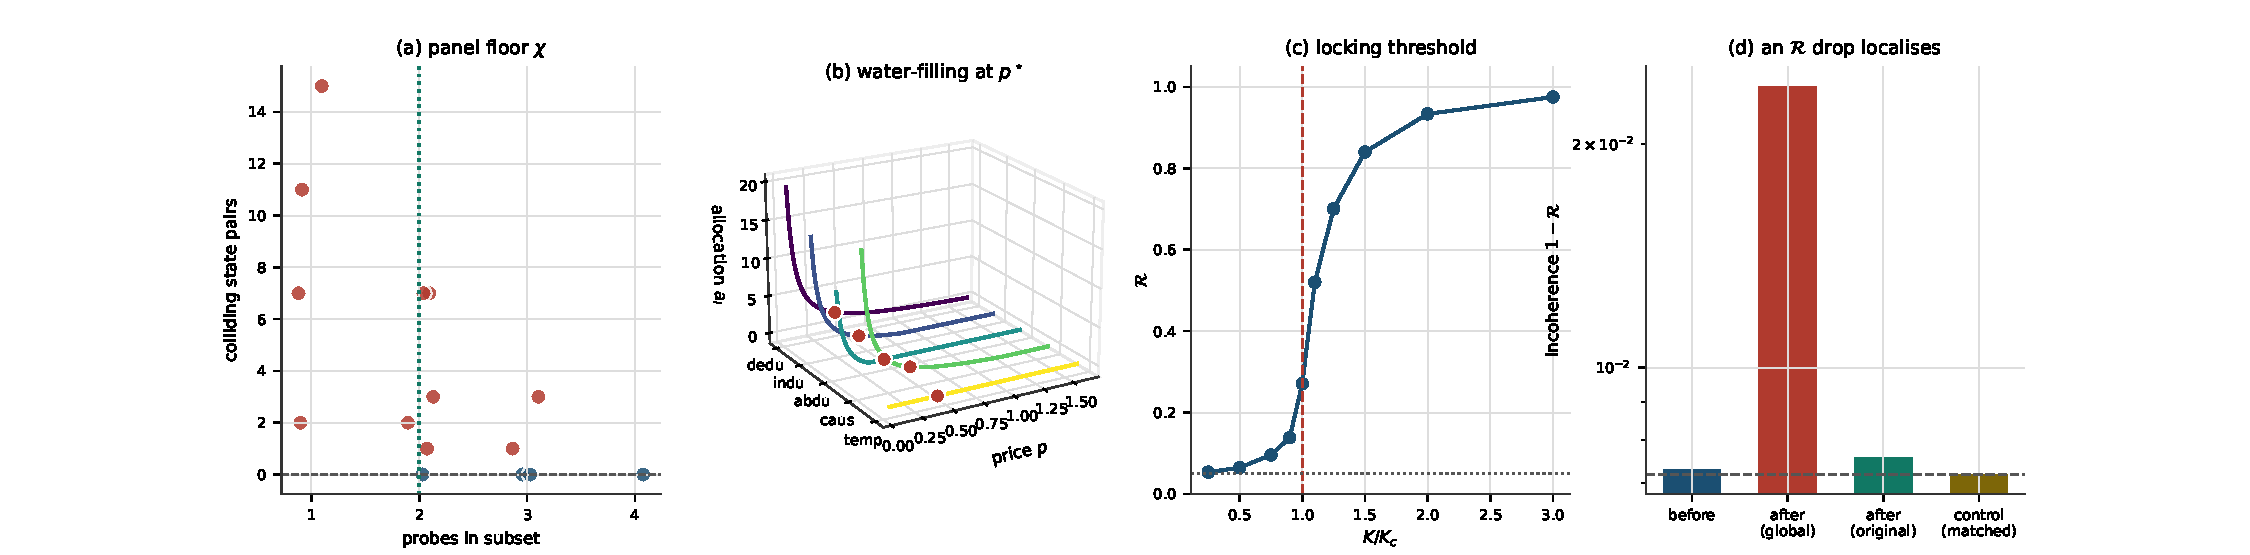
\includegraphics[width=\textwidth]{figures/panel_6_panel_layer.pdf}
    \caption{\textbf{The panel layer: a computed discrimination floor, graded allocation at one price, and a coordination threshold that is derived rather than assumed.}
    (\textbf{A})~Colliding state pairs against subset size, over all $15$ subsets of the four observables applied to the seven-state cycle at a resolving power of \SI{4}{\nano\metre}. Subsets reaching zero collisions (blue) are exactly those that separate the whole state set, with no exceptions in either direction --- \Cref{thm:discrimination} holds without qualification. The floor is $\chi = 2$, attained uniquely by $\{\text{M\"ossbauer},\ \text{UV--Vis}\}$, and the vertical rule marks it. Size alone does not determine separation: some three-element subsets still collide while a two-element subset succeeds, so what buys resolution is disjointness of what the observables see, not how many are deployed. The floor asserted by the earlier reading of \Cref{cor:three} does not survive; we report the computed value rather than adjusting the state table until three came out, per \Cref{rem:floor-computed}.
    (\textbf{B})~Water-filling. Allocation against price for five reasoners, with the solution at the single shadow price $p^\star = 0.432$ marked (budget $B = 4.0$; KKT residual $5.6\times10^{-17}$, agreeing with an independent optimiser to $9.7\times10^{-8}$). Three reasoners are engaged at graded, unequal allocations; two sit at the dropout boundary $\gamma'(0) \le p^\star$ of \Cref{cor:graded} rather than being excluded by a separate rule. Dropout is a boundary case of one law, not a second mechanism.
    (\textbf{C})~The locking threshold of \Cref{thm:lock}. Order parameter $\mathcal{R}$ against $K/K_c$ for $M = 400$ oscillators at $\sigma = 0.5$, where $K_c = 2/\pi g(\bar\omega) = 0.798$ is \emph{computed} from the observed frequency spread rather than fitted to the curve. The transition occurs at the predicted location, and $\mathcal{R}$ rests on the finite-$M$ incoherent floor $1/\sqrt{M} = 0.05$ (dotted) below it. Coordination is thus a threshold phenomenon with a derived critical point, not an assumed agreement.
    (\textbf{D})~Localisation, plotted as incoherence $1-\mathcal{R}$ on a logarithmic axis because the entire effect lies in the third decimal and is invisible on a $[0,1]$ scale. Admitting one mismatched newcomer to a panel of $M = 60$ drops the global order parameter from $0.99270$ to $0.97605$, while the order parameter restricted to the original members is essentially unmoved at $0.99244$, and the matched-newcomer control does not drop at all ($0.99282$). The dashed line is the bound $(M\mathcal{R}_{\text{old}}+1)/(M+1)$ of \Cref{prop:localisation}, which holds. The drop localises to the newcomer: it is evidence about the arrival, not about the panel.}
    \label{fig:panel6}
\end{figure*}
